\section{Einleitung und Zielsetzung}
\begin{wrapfigure}{r}{0.3\textwidth}
	\centering
	\vspace{-10pt}
	\framebox[0.3\textwidth]{
	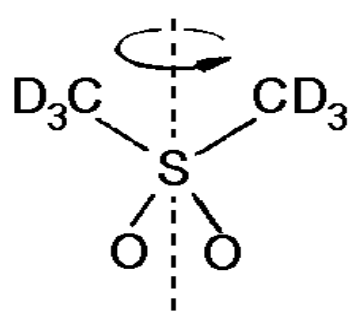
\includegraphics[width=0.25\textwidth]{Plots/Probe.png} }
	\caption{Di{\-}me{\-}thyl{\-}sul{\-}fon-Kristall (siehe Versuchsanleitung \cite{Anleitung}[S.2]).}
	\label{probe}
\end{wrapfigure}
In diesem Versuch soll mittels magnetischer Kernresonanz (NMR) Spektroskopie die Molek\"{u}l- und Ionendynamik der vorliegenden Pulver-Probe untersucht werden.
Diese Probe besitzt unz\"{a}hlige isotrop orientierte Kristalle (Dimethylsulfon-Kristalle, siehe Abbildung (\ref{probe})).
Die Untersuchungen werden mit einem Deuteronen-NMR durchgef\"{u}hrt.
Mit der magnetische Kernresonanz k\"{o}nnen unteranderem Informationen \"{u}ber dynamische Bewegungspro{\-}zesse ermittelt werden.
Ziel dieses Versuches ist es, die Relaxationszeiten $T_1$ und $T_2$ der vorliegenden Probe zu bestimmen.
Sowie stimulierte Echos f\"{u}r verschiedene Temperaturen aufzunehmen.
